%In this chapter you have to concisely explain the problem that you want to solve and the goal of your solution. This part should contain:

% 1) Detailed analysis of the problem and its limitations (e.g. what is the bottleneck and difficulties).

% 2) Your research methods – how did you identify these problems (e.g. tools used)?

% 3) You should clearly state and explain your goal and objectives. You should provide analytical study (mathematical model) of your solution (What is the upper and lower bound of your performance or improvements). You should also mention about the qualitative benefit of your solution such as easy programming etc..

% If necessary you may divide this chapter in sections and subsections.

\subsection*{Motivation}
%TODO rewrite O'Reilly 
%TODO add bidirectional (it could be that neurons in brain are connected that way) 

\subsubsection{O'Reilly} 
It corresponds to O'Reillys motivations \cite{o1998six}.

O'Reilly presents what he thinks as biologically plausible. In the end of this review we provide citations from this article which shortly explain the most important concepts of NN design. 

Article also contains interesting references to several experiments. It also presents the Leabra model (PhD thesis of O'Reilly) which is presented as a base model for other NN which can be derived from Leabra. The question how to merge the proposed principles is dicussed, especially the case of competiveness and distributed representation. 

\paragraph{Biological realism.} Moreover, computational mechanisms that violate
known biological properties should not be relied upon. 

A criticism of back-propagation is that it is neurally implausible (and hard to implement in hardware) because it requires all the connections to be used backward and it requires the units to use different input-output functions for the forward and backward passes \cite{hinton1988learning}.

\paragraph{Distributed representations.} A distributed representation
uses multiple active neuron-like processing units to encode
information (as opposed to a single unit, localist represen-
tation), and the same unit can participate in multiple repre-
sentations. Each unit in a distributed representation can be
thought of as representing a single feature, with information
being encoded by particular combinations of such features \cite{hinton1988learning}.

\paragraph{Inhibitory competition.} Inhibitory competition arises when mutual
inhibition among a set of units (i.e. as mediated by in-
hibitory interneurons) prevents all but a subset of them
from becoming active at a time.  Furthermore, most learn-
ing mechanisms (including those discussed later) are
affected by this selection process such that only the selected
representations are refined over time through learning, re-
sulting in an effective differentiation and distribution of
representations. More generally, it seems as though the world can be usefully
represented in terms of a large number of categories with a
large number of exemplars per category (animals, furniture,
trees, etc.) \cite{hinton1988learning}. 

\paragraph{Bidirectional activation propagation (interactivity).} They showed that
interactivity could explain the counterintuitive finding that
higher-level word processing can influence lower-level letter
perception. More recently, Vecera and O’Reilly showed
that bidirectional constraint satisfaction can model people’s
ability to resolve ambiguous visual inputs in favor of familiar
versus novel objects \cite{hinton1988learning}. 

\paragraph{Error-driven task learning.} Error-driven learning (also called ‘supervised’ learning) is
important for shaping representations according to task de-
mands by learning to minimize the difference (i.e. the error)
between a desired outcome and what the network actually
produced \cite{hinton1988learning}. 

\paragraph{Hebbian model learning.} That something like correlational structure is important.
Hebbian learning mechanisms represent this correlational
structure, encoding the extent to which different things co-
occur in the environment \cite{hinton1988learning}.

\subsubsection{Da} 

\cite{da2011advances} 

There is evidence that the cerebral cortex is connected in a
bi-directional way and distributed representations prevail in
it \cite{o2000computational}. So, more biologically plausible connectionist models
should present some of the following characteristics \cite{orru2008sabio}:

\paragraph{Distributed representation.} Generalization and reduction
of the network size can be obtained if the adopted
representation is distributed, since connections among
units are able to support a large number of different
patterns and create new concepts without allocation of
new hardware;

\paragraph{Inhibitory competition.} Neurons that are next to the
“winner” neuron receive a negative stimulus, strengthen-
ing the winner neuron (a kind of winner-takes-all). Dur-
ing a lateral inhibition, a neuron excites an inhibitory
inter-neuron that makes a feed-back connection on the
first neuron \cite{o1998six};

\paragraph{Bi-directional activation propagation.} Hidden layers re-
ceive stimuli from the input layer and from the output
layer. The bi-directionality of the architecture is neces-
sary to simulate a biological electrical synapse, which
can be bi-directional \cite{kandel1995essentials}, \cite{rosa2002biologically};

\paragraph{Error-driven task learning.} In GeneRec, the error is
calculated considering the local difference in synapses,
based on neurophysiological properties \cite{o1998six}, in contrast
to back-propagation, which requires error signals prop-
agate from the output layer towards the input layer.

\subsubsection{Usage} 

BioAnt \cite{schneider2009application} 
Cells \cite{nawrocki2012monitoring} 


\subsubsection{Other} 
\paragraph{Hebbian nature.}
%TODO make it a lot shorter 
%TODO: Read and cite from Hebbs's original article (Hebb, D.O. (1949). The organization of behavior. New York: Wiley \& Sons). 

(Wiki) Hebbian theory is a scientific theory in biological neuroscience which explains the adaptation of neurons in the brain during the learning process. It describes a basic mechanism for synaptic plasticity wherein an increase in synaptic efficacy arises from the presynaptic cell's repeated and persistent stimulation of the postsynaptic cell. Introduced by Donald Hebb in 1949, it is also called Hebb's rule, Hebb's postulate, and cell assembly theory, and states:

    "Let us assume that the persistence or repetition of a reverberatory activity (or "trace") tends to induce lasting cellular changes that add to its stability. When an axon of cell A is near enough to excite a cell B and repeatedly or persistently takes part in firing it, some growth process or metabolic change takes place in one or both cells such that A's efficiency, as one of the cells firing B, is increased."

The theory is often summarized as "Cells that fire together, wire together.".[1] It attempts to explain "associative learning", in which simultaneous activation of cells leads to pronounced increases in synaptic strength between those cells. Such learning is known as Hebbian learning.

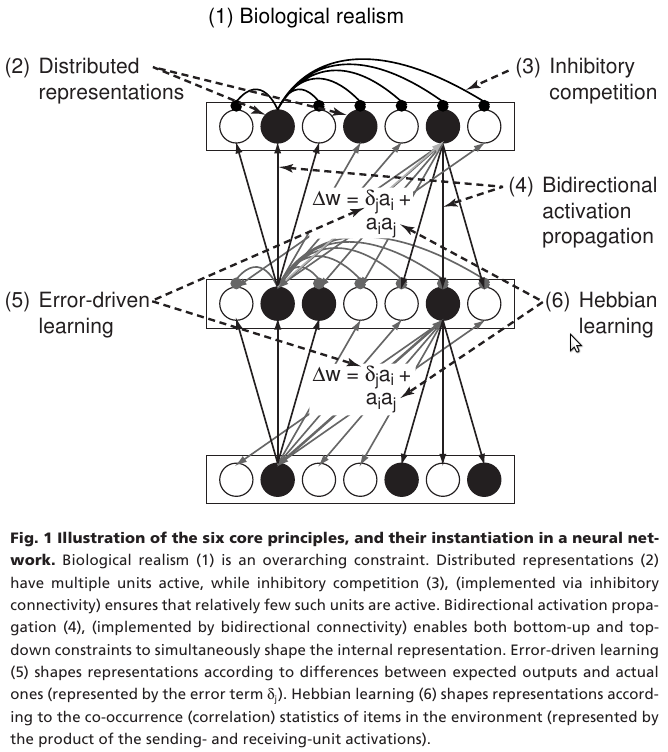
\includegraphics[width=12cm]{img/bio_plausability_o1998six.png}
